\section{详细设计}
\subsection{数据库设计}

\subsubsection{实体定义}
规范化数据层包含用户(User)、公司(Company)、职位(Job)和地址(Address)四个核心实体。这些实体严格遵循第三范式设计,消除数据冗余,保证数据一致性。用户实体用于系统访问控制,支持普通用户和管理员两种角色,确保系统安全;公司实体规范化存储招聘企业的基本信息,通过唯一的公司名称避免重复;职位实体以标准化格式记录招聘信息,通过外键关联到发布公司;地址实体则规范化存储地理位置信息,支持地理空间查询。实体之间通过关联关系表维护多对多关系,形成完整且规范的数据模型。表\ref{tab:entity_definition}详细说明了规范化数据层各实体的定义:

\begin{table}[htbp]
  \centering
  \caption{系统实体定义}
  \label{tab:entity_definition}
  \begin{tabular}{|p{0.15\textwidth}|p{0.35\textwidth}|p{0.4\textwidth}|}
    \hline
    \begin{center}\textbf{实体名称}\end{center} & \begin{center}\textbf{主要属性}\end{center} & \begin{center}\textbf{说明}\end{center} \\
    \hline
    \multirow{5}{*}{用户(User)} & 
    \begin{itemize}
      \item 用户ID(主键)
      \item 用户名
      \item 密码
      \item 用户角色
      \item 创建时间
    \end{itemize} & 
    \begin{center}系统用户信息,支持基本的角色权限控制。用户可以分为普通用户和管理员两种角色,用于管理系统访问权限。\end{center} \\
    \hline
    \multirow{6}{*}{公司(Company)} & 
    \begin{itemize}
      \item 公司ID(主键)
      \item 公司名称(唯一)
      \item 所属行业
      \item 公司规模
      \item 创建时间
      \item 更新时间
    \end{itemize} & 
    \begin{center}招聘公司的基本信息。公司名称需要保持唯一性以避免重复,通过所属行业和公司规模等属性可以支持多维度的分析查询。\end{center} \\
    \hline
    \multirow{11}{*}{职位(Job)} & 
    \begin{itemize}
      \item 职位ID(主键)
      \item 职位名称
      \item 职位类型
      \item 薪资范围
      \item 经验要求
      \item 学历要求
      \item 技能要求
      \item 职位福利
      \item 数据来源
      \item 创建时间
      \item 更新时间
    \end{itemize} & 
    \begin{center}职位发布的详细信息。包含职位要求、待遇等完整招聘信息,通过数据来源字段可以追踪数据来源渠道。\end{center} \\
    \hline
    \multirow{6}{*}{地址(Address)} & 
    \begin{itemize}
      \item 地址ID(主键)
      \item 地址文本
      \item 经度
      \item 纬度
      \item 创建时间
      \item 更新时间
    \end{itemize} & 
    \begin{center}公司和职位关联的地理位置信息。通过经纬度坐标支持地理位置检索和距离计算,可用于就近推荐等功能。\end{center} \\
    \hline
  \end{tabular}
\end{table}

图\ref{fig:normalized_data_er}展示了规范化数据层的数据结构设计。该设计严格遵循第三范式(3NF),通过实体表和关系表的合理组织,消除了数据冗余,保证了数据一致性。该E-R图清晰地展示了系统中各实体之间的关联关系,为后续的物理设计和系统实现提供了重要指导。下面是关于图中的实体表User、Company、Job和Address和关系表company\_address、job\_address的详细说明。

\begin{figure}[htbp]
  \centering
  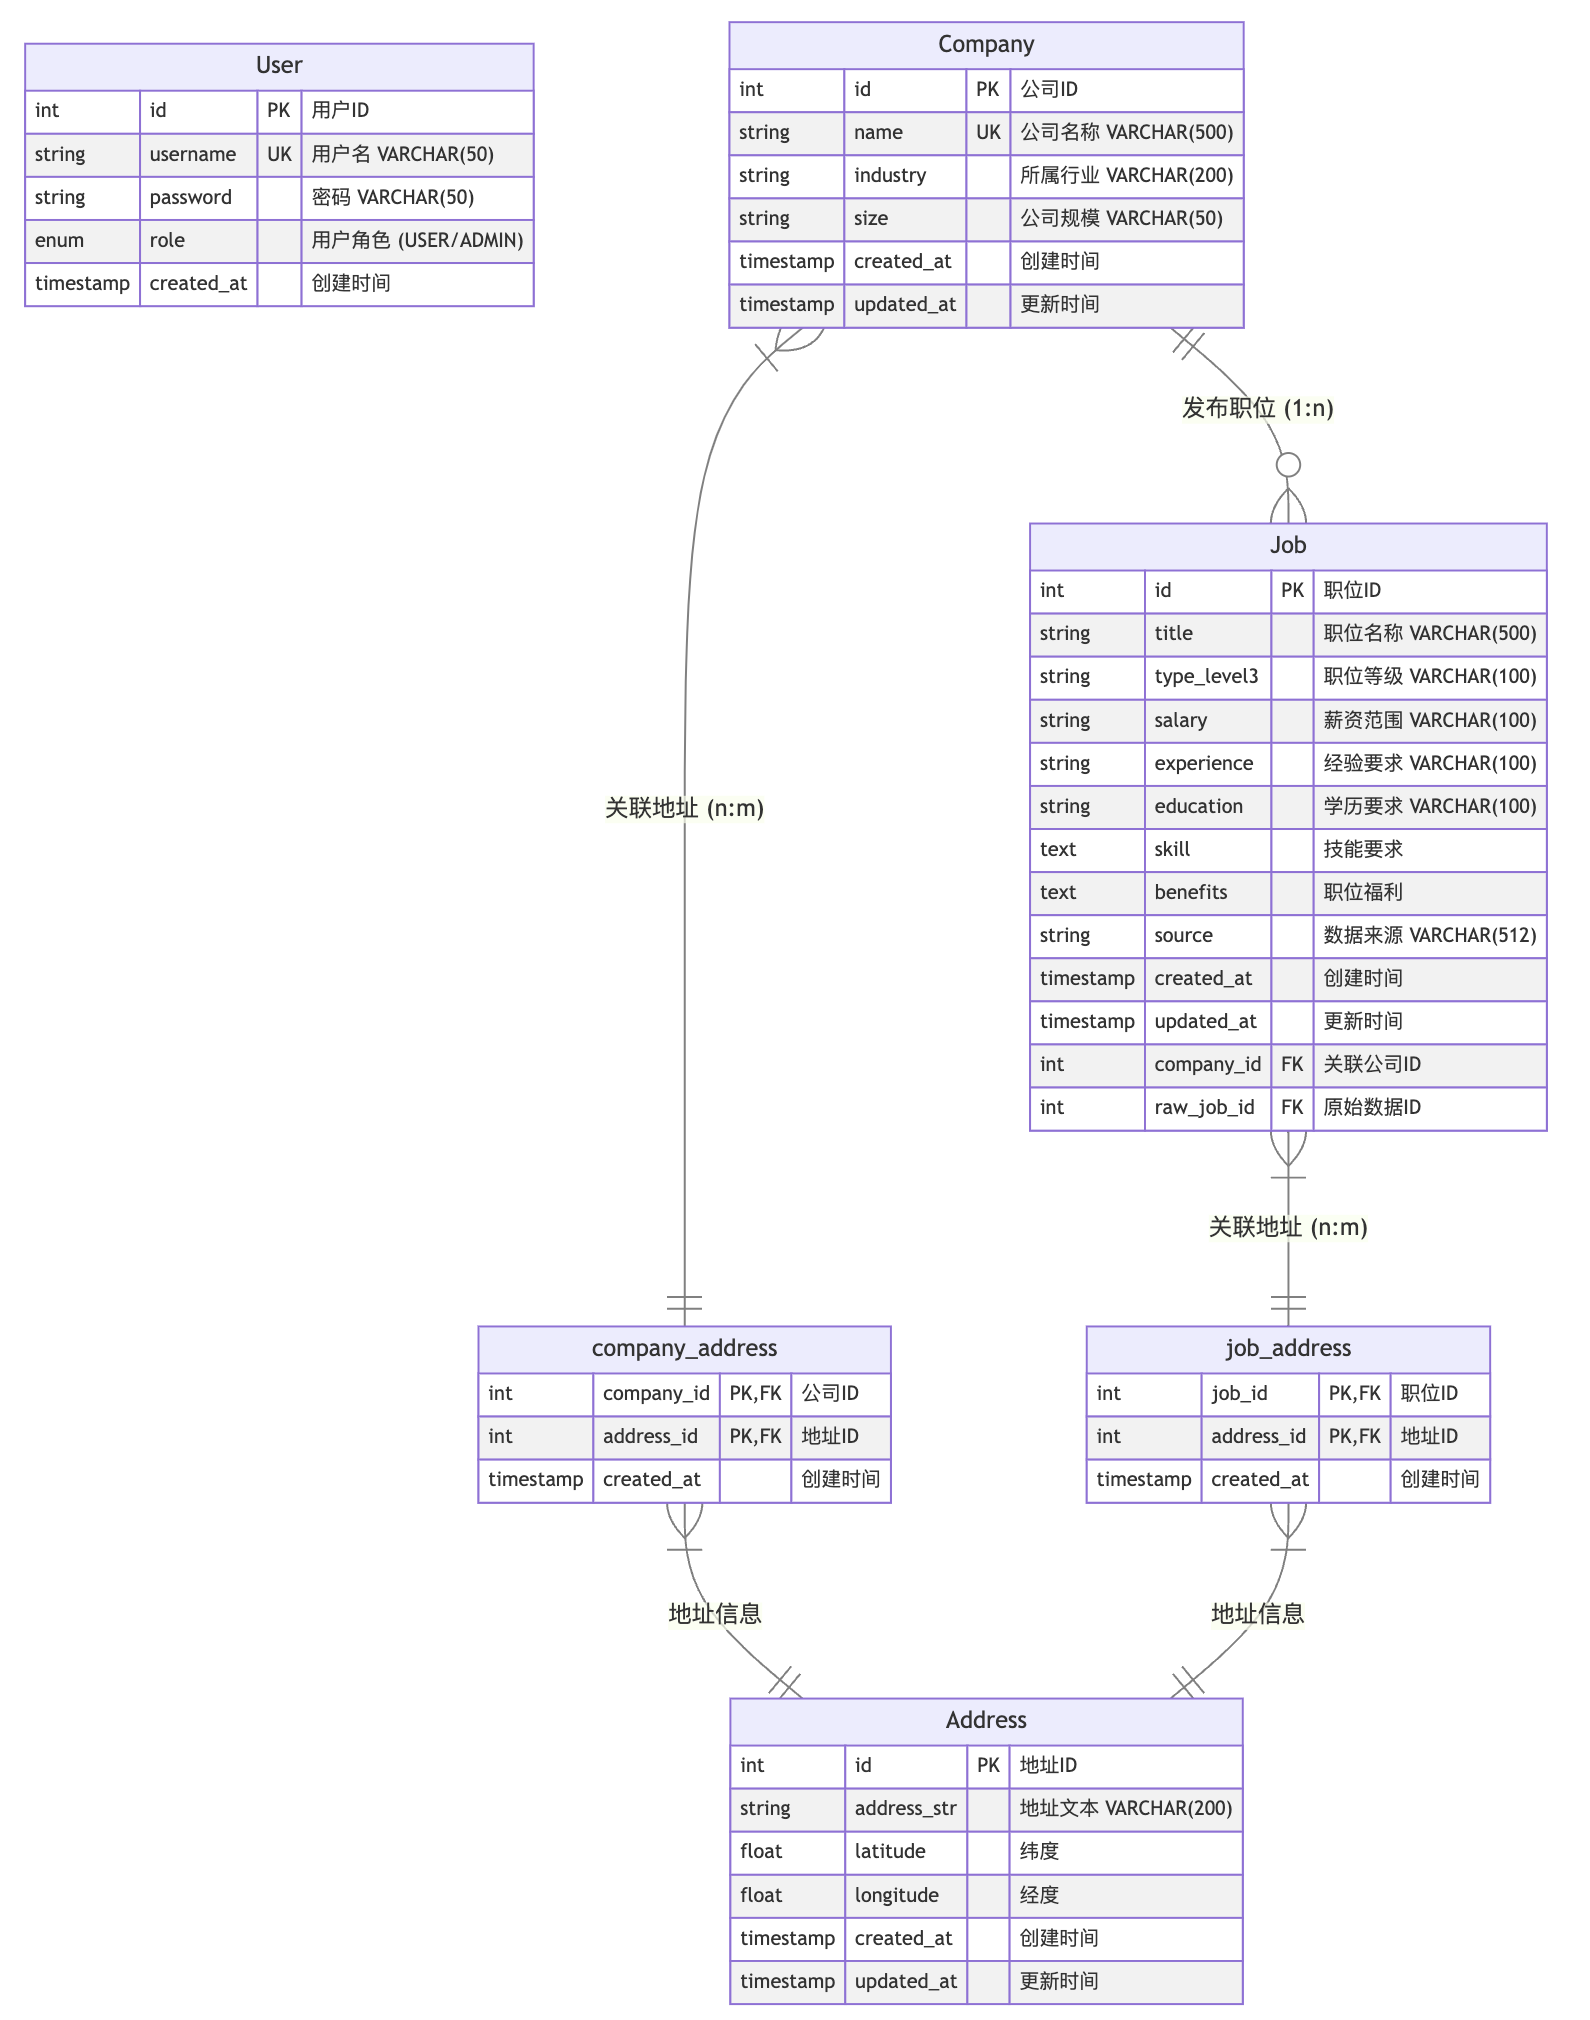
\includegraphics[width=0.8\textwidth]{figures/数据库实体ER图.png}
  \caption{规范化数据层E-R图}
  \label{fig:normalized_data_er}
\end{figure}


\paragraph{核心实体表设计}
系统的数据模型主要由四个基本实体表构成,每个实体表都严格遵循第三范式(3NF)设计原则。用户(User)表作为系统的基础用户管理单元,存储用户的身份认证和授权信息。该表包含用户ID作为主键,用户名设置唯一约束,同时存储密码和用户角色信息。通过角色字段(枚举类型:user/admin)实现基本的权限管理,并在用户名上建立索引(ix\_users\_username)以优化登录查询性能。

公司(Company)表存储招聘公司的核心信息,是职位信息的关联主体。该表以公司ID为主键,公司名称设置唯一约束,同时包含所属行业、公司规模等基本信息字段。为支持多维度的查询需求,表中建立了针对性的复合索引,包括公司名称索引(ix\_companies\_name)、行业规模复合索引(ix\_companies\_industry\_size)以及名称行业复合索引(ix\_companies\_name\_industry)。

职位(Job)表作为系统的核心业务实体,存储完整的招聘信息。除职位ID主键外,该表包含职位名称、类型、薪资范围、经验要求、学历要求等详细信息。通过company\_id外键与公司表建立关联,实现一对多关系,同时通过raw\_job\_id关联到暂存数据表保证数据可追溯性。该表设计了多个针对性索引,包括职位名称索引(ix\_jobs\_title)、公司关联索引(ix\_jobs\_company\_id)等,以优化不同场景下的查询性能。

地址(Address)表统一管理地理位置信息,支持地理空间查询功能。该表包含地址ID主键、地址文本、经纬度坐标等字段。特别值得注意的是,该表使用了PostgreSQL的GIN索引(ix\_addresses\_address\_str\_trgm)支持地址文本的模糊查询,并通过经纬度复合索引(ix\_addresses\_coordinates)支持地理位置检索和距离计算。

\paragraph{关系表设计}
为处理实体间的多对多关系,系统设计了两个关系表。公司-地址关联表(company\_address)通过复合主键(company\_id, address\_id)唯一标识每条关联记录,包含创建时间字段以支持关系建立时间的追踪。职位-地址关联表(job\_address)采用相同的复合主键设计,用于记录职位发布地点的多地址情况,支持按地理位置筛选职位的功能需求。这两个关系表都通过外键约束确保数据完整性和一致性。

\paragraph{实体关系说明}
系统中的实体关系构成了一个完整的业务闭环。公司与职位之间形成一对多(1:n)关系,通过Job表中的company\_id外键实现关联,确保每个职位都必须归属于一个有效的公司。公司与地址之间,以及职位与地址之间都是多对多(n:m)关系,分别通过company\_address和job\_address关系表实现。这种设计反映了现实中公司可能有多个办公地点,以及职位可能在多个地点同时招聘的场景,同时避免了数据冗余。

\paragraph{设计特点}
本设计通过主键和外键约束确保数据的引用完整性,所有实体和关系表都包含创建时间和更新时间字段以支持数据变更追踪。通过精心设计的索引策略,在查询性能和存储开销之间取得平衡。地理坐标和空间索引的设计支持了位置服务相关功能。同时,设计预留了适当的字段类型和长度,支持未来功能扩展。整体设计严格遵循3NF,通过实体表和关系表的合理组织,既消除了数据冗余,又保证了数据一致性。




\subsection{数据处理层设计}

\begin{enumerate}
  \item BOSS直聘原始数据(RawRecruitmentData\_Boss)
  \begin{itemize}
    \item 目的:存储BOSS直聘爬虫采集的原始数据
    \item 主要字段:
    \begin{itemize}
      \item 职位信息:标题、类型、薪资等
      \item 公司信息:名称、简介等
      \item 地址信息:地址文本
      \item 元数据:来源URL、原始数据JSON等
    \end{itemize}
  \end{itemize}

  \item 猎聘网原始数据(RawRecruitmentData\_Liepin)
  \begin{itemize}
    \item 目的:存储猎聘网爬虫采集的原始数据
    \item 主要字段:
    \begin{itemize}
      \item 职位信息:标题、薪资等
      \item 公司信息:名称、行业、规模等
      \item 地址信息:地址文本
      \item 元数据:标签列表、原始数据等
    \end{itemize}
  \end{itemize}

  \item 暂存数据(StagedRecruitmentData)
  \begin{itemize}
    \item 目的:统一格式,支持数据清洗和转换
    \item 主要字段:
    \begin{itemize}
      \item 统一后的职位信息
      \item 统一后的公司信息
      \item 统一后的地址信息
      \item 去重相关字段:记录哈希、重复组ID等
    \end{itemize}
  \end{itemize}
\end{enumerate}

\subsection{E-R图}

% \begin{figure}[htbp]
%   \centering
%   \includegraphics[width=0.8\textwidth]{figures/normalized_data_er.png}
%   \caption{规范化数据层E-R图}
%   \label{fig:normalized_er}
% \end{figure}

% \begin{figure}[htbp]
%   \centering
%   \includegraphics[width=0.8\textwidth]{figures/processing_data_er.png}
%   \caption{数据处理层E-R图}
%   \label{fig:processing_er}
% \end{figure}

数据处理层的实体关系(E-R)图\ref{fig:processing_er}展示了系统数据ETL过程中的数据结构设计,主要包含两类原始数据表和一个暂存数据表。这种设计支持数据的采集、清洗和转换过程,为规范化数据层提供数据基础。

\begin{figure}[htbp]
  \centering
  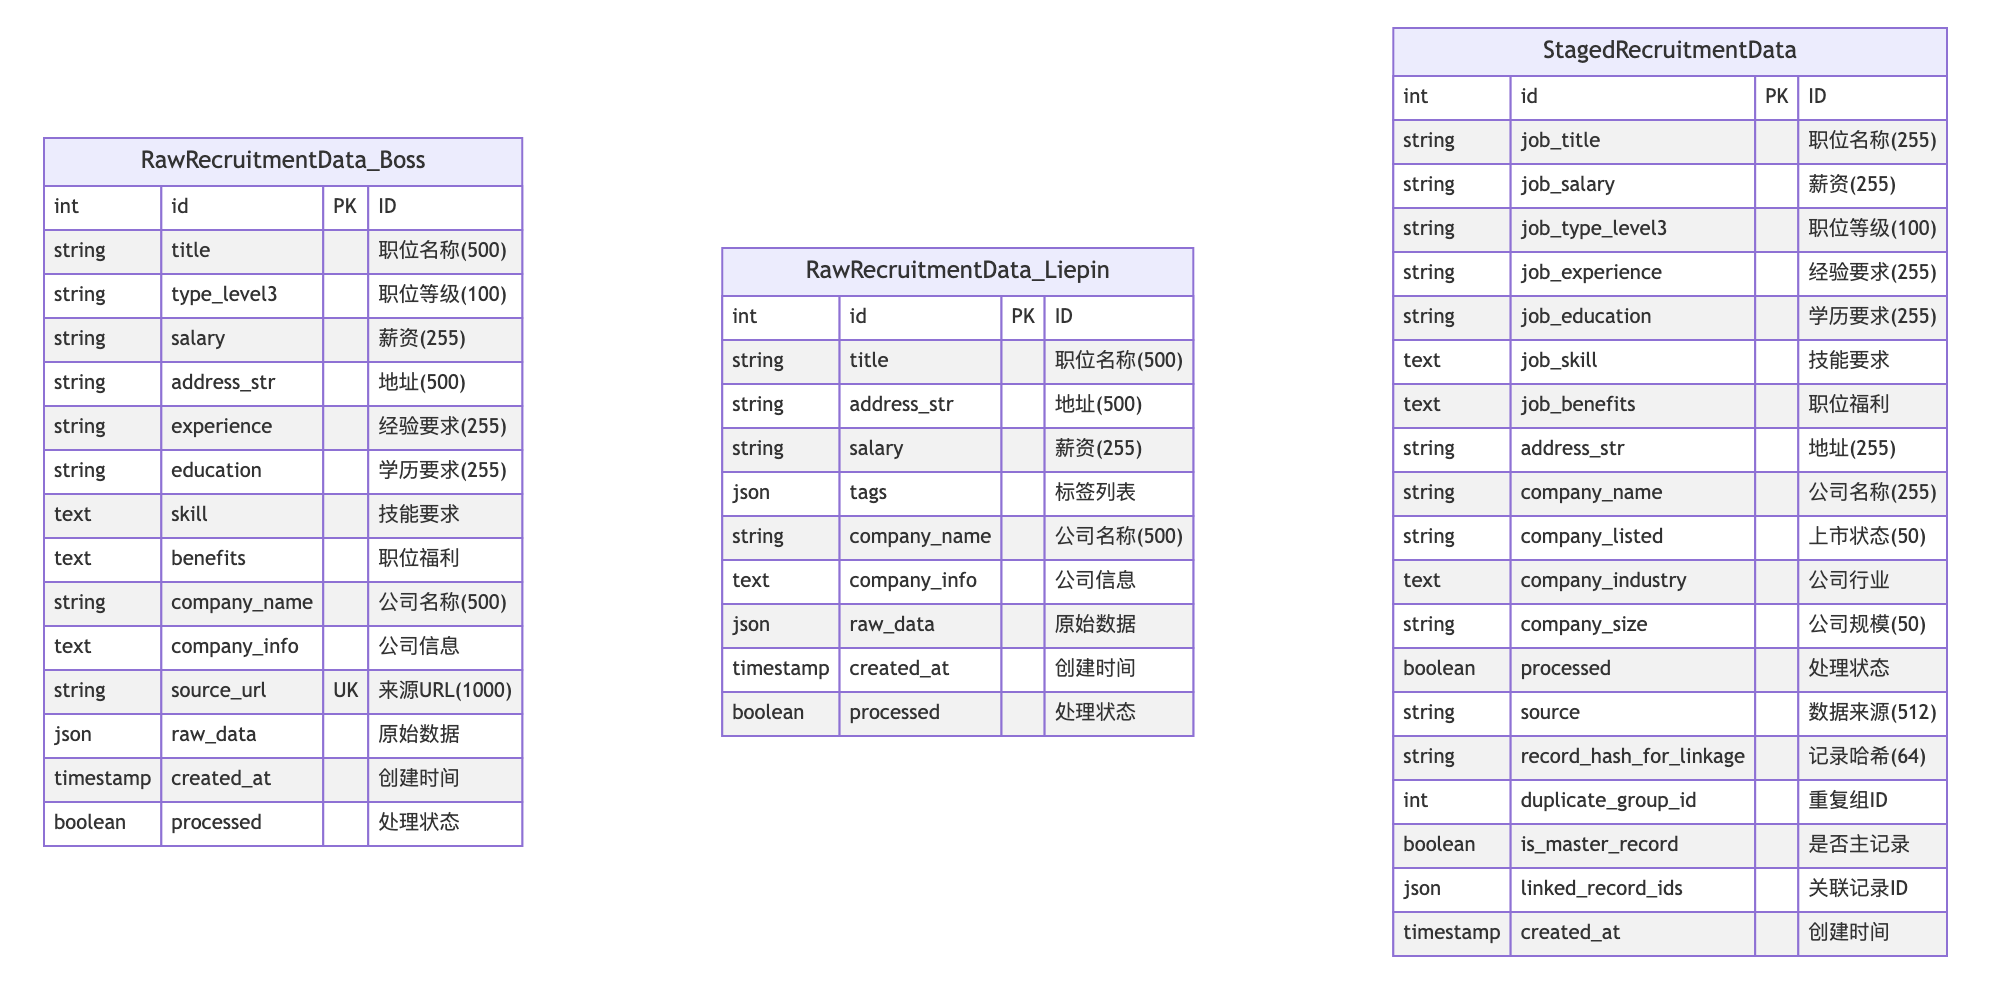
\includegraphics[width=0.8\textwidth]{figures/数据处理层ER图.png}
  \caption{数据处理层E-R图}
  \label{fig:processing_er}
\end{figure}

\paragraph{原始数据表设计}
如表\ref{tab:raw_boss_data_fields}和表\ref{tab:raw_liepin_data_fields}所示,系统包含两个原始数据表,分别对应不同的数据来源:

\begin{table}[htbp]
  \centering
  \caption{BOSS直聘原始数据表字段设计}
  \label{tab:raw_boss_data_fields}
  \begin{tabular}{@{}lll@{}}
    \toprule
    \textbf{字段类型} & \textbf{字段名} & \textbf{说明} \\
    \midrule
    \multirow{3}{*}{基础信息}
    & id & 主键 \\
    & created\_at & 创建时间 \\
    & processed & 处理状态标记 \\
    \midrule
    \multirow{7}{*}{职位信息}
    & job\_title & 职位名称(500字符) \\
    & job\_level & 职位等级(100字符) \\
    & salary & 薪资(255字符) \\
    & experience & 经验要求(255字符) \\
    & education & 学历要求(255字符) \\
    & skills & 技能要求(文本) \\
    & benefits & 职位福利(文本) \\
    \midrule
    \multirow{2}{*}{公司信息}
    & company\_name & 公司名称(500字符) \\
    & company\_detail & 公司详细信息(文本) \\
    \midrule
    \multirow{3}{*}{其他信息}
    & address & 地址文本(500字符) \\
    & source\_url & 来源URL(1000字符,唯一约束) \\
    & raw\_data & 原始数据(JSON) \\
    \bottomrule
  \end{tabular}
\end{table}

\begin{table}[htbp]
  \centering
  \caption{猎聘网原始数据表字段设计}
  \label{tab:raw_liepin_data_fields}
  \begin{tabular}{@{}lll@{}}
    \toprule
    \textbf{字段类型} & \textbf{字段名} & \textbf{说明} \\
    \midrule
    \multirow{3}{*}{基础信息}
    & id & 主键 \\
    & created\_at & 创建时间 \\
    & processed & 处理状态标记 \\
    \midrule
    \multirow{2}{*}{职位信息}
    & job\_title & 职位名称(500字符) \\
    & salary & 薪资(255字符) \\
    \midrule
    \multirow{2}{*}{公司信息}
    & company\_name & 公司名称(500字符) \\
    & company\_detail & 公司详细信息(文本) \\
    \midrule
    \multirow{3}{*}{其他信息}
    & address & 地址文本(500字符) \\
    & tags & 标签列表(JSON) \\
    & raw\_data & 原始数据(JSON) \\
    \bottomrule
  \end{tabular}
\end{table}

\paragraph{暂存数据表设计}
如表\ref{tab:staged_recruitment_data_fields}所示,暂存数据表(StagedRecruitmentData)作为数据清洗和转换的中间层:

\begin{table}[htbp]
  \centering
  \caption{暂存数据表字段设计}
  \label{tab:staged_recruitment_data_fields}
  \begin{tabular}{@{}lll@{}} 
    \toprule
    \textbf{字段类型} & \textbf{字段名} & \textbf{说明} \\ 
    \midrule
    \multirow{7}{*}{职位相关字段} 
    & job\_title & 职位名称(255字符) \\
    & job\_salary & 薪资描述(255字符) \\
    & job\_type\_level3 & 职位等级(100字符) \\
    & job\_experience & 经验要求(255字符) \\
    & job\_education & 学历要求(255字符) \\
    & job\_skill & 技能要求(文本) \\
    & job\_benefits & 职位福利(文本) \\
    \midrule
    \multirow{4}{*}{公司相关字段}
    & company\_name & 公司名称(255字符) \\
    & company\_listed & 上市状态(50字符) \\
    & company\_industry & 公司行业(文本) \\
    & company\_size & 公司规模(50字符) \\
    \midrule
    \multirow{6}{*}{数据处理相关字段}
    & processed & 处理状态标记(布尔值) \\
    & source & 数据来源标识(512字符) \\
    & record\_hash\_for\_linkage & 记录哈希值(64字符),用于快速判断重复 \\
    & duplicate\_group\_id & 重复记录组ID \\
    & is\_master\_record & 主记录标记(布尔值) \\
    & linked\_record\_ids & 关联记录ID列表(JSON) \\
    \bottomrule
  \end{tabular}
\end{table}

\subsection{关系模式设计}

\subsubsection{规范化数据层关系模式}

用户关系模式、公司关系模式、职位关系模式、地址关系模式、公司-地址关系模式、职位-地址关系模式的定义分别如代码\ref{lst:user_schema}-\ref{lst:job_address_schema}所示。


  \begin{listing}[htbp]
    \begin{minted}{sql}
User(
    id: Integer (PK),
    username: String(50) NOT NULL UNIQUE,
    password: String(50) NOT NULL,
    role: Enum('user', 'admin') NOT NULL DEFAULT 'user',
    created_at: DateTime NOT NULL
)
    \end{minted}
    \caption{用户表结构}\label{lst:user_schema}
  \end{listing}

  \begin{listing}[htbp]
    \begin{minted}{sql}
Company(
    id: Integer (PK),
    name: String(500) NOT NULL UNIQUE,
    industry: String(200),
    size: String(50),
    created_at: DateTime NOT NULL,
    updated_at: DateTime NOT NULL
)
    \end{minted}
    \caption{公司表结构}\label{lst:company_schema}
  \end{listing}

  \begin{listing}[htbp]
    \begin{minted}{sql}
Job(
    id: Integer (PK),
    title: String(500) NOT NULL,
    type_level3: String(100),
    salary: String(100),
    experience: String(100),
    education: String(100),
    skill: Text,
    benefits: Text,
    source: String(512),
    company_id: Integer (FK -> Company.id),
    raw_job_id: Integer (FK -> StagedRecruitmentData.id),
    created_at: DateTime NOT NULL,
    updated_at: DateTime NOT NULL
)
    \end{minted}
    \caption{职位表结构}\label{lst:job_schema}
  \end{listing}

  \begin{listing}[htbp]
    \begin{minted}{sql}
Address(
    id: Integer (PK),
    address_str: String(200) NOT NULL,
    latitude: Float,
    longitude: Float,
    created_at: DateTime NOT NULL,
    updated_at: DateTime NOT NULL
)
    \end{minted}
    \caption{地址表结构}\label{lst:address_schema}
  \end{listing}

  \begin{listing}[htbp]
    \begin{minted}{sql}
company_address(
    company_id: Integer (PK, FK -> Company.id),
    address_id: Integer (PK, FK -> Address.id),
    created_at: DateTime NOT NULL
)
    \end{minted}
    \caption{公司-地址关系表结构}\label{lst:company_address_schema}
  \end{listing}

  \begin{listing}[htbp]
    \begin{minted}{sql}
job_address(
    job_id: Integer (PK, FK -> Job.id),
    address_id: Integer (PK, FK -> Address.id),
    created_at: DateTime NOT NULL
)
    \end{minted}
    \caption{职位-地址关系表结构}\label{lst:job_address_schema}
  \end{listing}

\subsubsection{数据处理层关系模式}

BOSS直聘原始数据关系模式、猎聘网原始数据关系模式和暂存数据关系模式的定义分别如代码\ref{lst:raw_boss_schema}-\ref{lst:staged_data_schema}所示。

  \begin{listing}[htbp]
    \begin{minted}{sql}
RawRecruitmentData_Boss(
    id: Integer (PK),
    title: String(500),
    type_level3: String(100),
    salary: String(255),
    address_str: String(500),
    experience: String(255),
    education: String(255),
    skill: Text,
    benefits: Text,
    company_name: String(500),
    company_info: Text,
    source_url: String(1000) UNIQUE,
    raw_data: JSON,
    created_at: DateTime NOT NULL,
    processed: Boolean DEFAULT FALSE
)
    \end{minted}
    \caption{BOSS直聘原始数据表结构}\label{lst:raw_boss_schema}
  \end{listing}

  \begin{listing}[htbp]
    \begin{minted}{sql}
RawRecruitmentData_Liepin(
    id: Integer (PK),
    title: String(500),
    address_str: String(500),
    salary: String(255),
    tags: JSON,
    company_name: String(500),
    company_info: Text,
    raw_data: JSON,
    created_at: DateTime NOT NULL,
    processed: Boolean DEFAULT FALSE
)
    \end{minted}
    \caption{猎聘网原始数据表结构}\label{lst:raw_liepin_schema}
  \end{listing}

  \begin{listing}[htbp]
    \begin{minted}{sql}
StagedRecruitmentData(
    id: Integer (PK),
    job_title: String(255),
    job_salary: String(255),
    job_type_level3: String(100),
    job_experience: String(255),
    job_education: String(255),
    job_skill: Text,
    job_benefits: Text,
    address_str: String(255),
    company_name: String(255),
    company_listed: String(50),
    company_industry: Text,
    company_size: String(50),
    source: String(512),
    record_hash_for_linkage: String(64),
    duplicate_group_id: Integer,
    is_master_record: Boolean DEFAULT FALSE,
    linked_record_ids: JSON,
    processed: Boolean DEFAULT FALSE,
    created_at: DateTime NOT NULL
)
    \end{minted}
    \caption{暂存数据表结构}\label{lst:staged_data_schema}
  \end{listing}

\subsection{完整性约束设计}

\subsubsection{实体完整性约束}

\begin{enumerate}
  \item 主键约束
  \begin{itemize}
    \item 所有表都使用自增整数id作为主键,确保每条记录的唯一标识
    \item 关系表使用联合主键:
    \begin{itemize}
      \item company\_address表使用(company\_id, address\_id)作为联合主键
      \item job\_address表使用(job\_id, address\_id)作为联合主键
      \item 联合主键可以防止重复关联关系的产生
    \end{itemize}
  \end{itemize}

  \item 唯一性约束
  \begin{itemize}
    \item User表的username字段设置唯一约束,确保用户名不重复
    \item Company表的name字段设置唯一约束,避免重复录入公司信息
    \item RawRecruitmentData\_Boss表的source\_url字段设置唯一约束,防止重复爬取
    \item StagedRecruitmentData表的record\_hash\_for\_linkage字段设置唯一约束,用于数据去重
  \end{itemize}
\end{enumerate}

\subsubsection{参照完整性约束}

\begin{enumerate}
  \item 外键约束设计
  
  数据库中的外键约束主要体现在三个方面:Job表与Company表及StagedRecruitmentData表的关联、company\_address关系表的双向关联、以及job\_address关系表的双向关联。如\cref{lst:foreign_keys}所示,这些外键约束确保了数据的引用完整性。其中,Job表通过company\_id关联到Company表,通过raw\_job\_id关联到StagedRecruitmentData表;company\_address表通过company\_id和address\_id分别关联到Company表和Address表;job\_address表则通过job\_id和address\_id分别关联到Job表和Address表。

  \begin{listing}[htbp]
    \begin{minted}{sql}
-- Job表的外键约束
ALTER TABLE Job ADD CONSTRAINT fk_job_company
    FOREIGN KEY (company_id) REFERENCES Company(id);
ALTER TABLE Job ADD CONSTRAINT fk_job_staged
    FOREIGN KEY (raw_job_id) REFERENCES StagedRecruitmentData(id);

-- company_address表的外键约束
ALTER TABLE company_address ADD CONSTRAINT fk_company_address_company
    FOREIGN KEY (company_id) REFERENCES Company(id);
ALTER TABLE company_address ADD CONSTRAINT fk_company_address_address
    FOREIGN KEY (address_id) REFERENCES Address(id);

-- job_address表的外键约束
ALTER TABLE job_address ADD CONSTRAINT fk_job_address_job
    FOREIGN KEY (job_id) REFERENCES Job(id);
ALTER TABLE job_address ADD CONSTRAINT fk_job_address_address
    FOREIGN KEY (address_id) REFERENCES Address(id);
    \end{minted}
    \caption{外键约束定义}\label{lst:foreign_keys}
  \end{listing}

  \item 级联操作策略
  
  为了确保数据的安全性和一致性,所有外键约束均采用RESTRICT策略。这意味着当尝试删除被其他表引用的记录时,数据库将阻止该操作(ON DELETE RESTRICT);同样,当尝试更新被引用的主键值时,也会被阻止(ON UPDATE RESTRICT)。系统不采用级联删除(CASCADE)机制,以防止因误操作导致大规模的数据丢失。所有需要进行的更新操作都通过应用层代码严格控制,以确保数据的一致性和完整性。
\end{enumerate}

\subsubsection{用户定义完整性约束}
对于用户定义完整性约束,主要包含三类约束:非空约束、默认值约束和检查约束。非空约束(如\cref{lst:not_null_constraints}所示)主要应用于User表的username、password和role字段,Company表的name字段,Job表的title和company\_id字段,以及Address表的address\_str字段,确保这些关键字段不能为空。默认值约束(如\cref{lst:default_constraints}所示)设置了User表role字段的默认值为'user',各数据处理表的processed字段默认值为FALSE,以及Company表和User表的时间戳字段默认值为当前时间。检查约束(如\cref{lst:check_constraints}所示)则对数据的有效性进行验证,包括User表role字段的取值范围限制,Address表经纬度的有效范围检查,以及Company表和Job表的时间戳先后顺序验证。

\begin{listing}[htbp]
    \begin{minted}{sql}
-- User表非空约束
ALTER TABLE User MODIFY username VARCHAR(50) NOT NULL;
ALTER TABLE User MODIFY password VARCHAR(50) NOT NULL;
ALTER TABLE User MODIFY role ENUM('user', 'admin') NOT NULL;

-- Company表非空约束
ALTER TABLE Company MODIFY name VARCHAR(500) NOT NULL;

-- Job表非空约束
ALTER TABLE Job MODIFY title VARCHAR(500) NOT NULL;
ALTER TABLE Job MODIFY company_id INTEGER NOT NULL;

-- Address表非空约束
ALTER TABLE Address MODIFY address_str VARCHAR(200) NOT NULL;
    \end{minted}
    \caption{非空约束定义}\label{lst:not_null_constraints}
  \end{listing}

\begin{listing}[htbp]
    \begin{minted}{sql}
-- 角色默认值
ALTER TABLE User ALTER role SET DEFAULT 'user';

-- 处理状态默认值
ALTER TABLE RawRecruitmentData_Boss ALTER processed SET DEFAULT FALSE;
ALTER TABLE RawRecruitmentData_Liepin ALTER processed SET DEFAULT FALSE;
ALTER TABLE StagedRecruitmentData ALTER processed SET DEFAULT FALSE;

-- 时间戳默认值
ALTER TABLE User ALTER created_at SET DEFAULT CURRENT_TIMESTAMP;
ALTER TABLE Company ALTER created_at SET DEFAULT CURRENT_TIMESTAMP;
ALTER TABLE Company ALTER updated_at SET DEFAULT CURRENT_TIMESTAMP;
    \end{minted}
    \caption{默认值约束定义}\label{lst:default_constraints}
  \end{listing}

\begin{listing}[htbp]
    \begin{minted}{sql}
-- 角色检查
ALTER TABLE User ADD CONSTRAINT check_user_role 
    CHECK (role IN ('user', 'admin'));

-- 经纬度范围检查
ALTER TABLE Address ADD CONSTRAINT check_latitude
    CHECK (latitude BETWEEN -90 AND 90);
ALTER TABLE Address ADD CONSTRAINT check_longitude
    CHECK (longitude BETWEEN -180 AND 180);

-- 时间戳有效性检查
ALTER TABLE Company ADD CONSTRAINT check_company_timestamps
    CHECK (updated_at >= created_at);
ALTER TABLE Job ADD CONSTRAINT check_job_timestamps
    CHECK (updated_at >= created_at);
    \end{minted}
    \caption{检查约束定义}\label{lst:check_constraints}
  \end{listing}

  \subsection{存储结构设计}

  \subsubsection{数据库选型}
  \begin{itemize}
    \item 选用PostgreSQL 数据库系统
    \begin{itemize}
      \item 支持JSON类型,用于存储爬虫原始数据(raw\_data字段)和地址聚合(addresses字段)
      \item 支持物化视图,用于预计算recruitment\_mv,提升查询性能
      \item 支持gin\_trgm\_ops操作符,用于地址和公司名称的模糊匹配
      \item 支持异步SQLAlchemy,实现高并发数据处理
      \item 内置的MVCC机制,保证数据一致性
    \end{itemize}
    \item 数据库配置
    \begin{itemize}
      \item 连接池:使用SQLAlchemy的异步会话管理
      \item 环境变量:通过.env文件配置数据库连接参数
      \item 时区处理:统一使用UTC时区存储时间戳
    \end{itemize}
  \end{itemize}
  
  \subsubsection{表空间组织}
  
  \begin{enumerate}
    \item 规范化数据层表空间
    \begin{itemize}
      \item 核心业务表:users, companies, jobs, addresses
      \begin{itemize}
        \item users表:用户认证和权限管理
        \item companies表:公司基本信息和元数据
        \item jobs表:职位详情和关联信息
        \item addresses表:地理位置和坐标数据
      \end{itemize}
      \item 关系映射表:company\_address, job\_address
      \begin{itemize}
        \item company\_address:多对多关系,支持一个公司多个地址
        \item job\_address:多对多关系,支持一个职位多个工作地点
      \end{itemize}
      \item 物化视图:recruitment\_mv
      \begin{itemize}
        \item 预聚合职位、公司、地址信息
        \item 支持高性能的分页和统计查询
        \item 定时刷新保证数据一致性
      \end{itemize}
    \end{itemize}
  
    \item 数据处理层表空间
    \begin{itemize}
      \item 原始数据表:raw\_recruitment\_boss, raw\_recruitment\_liepin
      \begin{itemize}
        \item 存储爬虫直接获取的JSON数据
        \item 使用processed标志位跟踪处理状态
        \item 保留source\_url确保数据不重复爬取
      \end{itemize}
      \item 暂存数据表:staged\_recruitment\_data
      \begin{itemize}
        \item 统一格式的中间表,存储清洗后的数据
        \item 支持跨来源的记录去重和链接
        \item 使用record\_hash\_for\_linkage优化相似度计算
        \item 通过duplicate\_group\_id和is\_master\_record管理重复记录
      \end{itemize}
    \end{itemize}
  \end{enumerate}
  
  \subsubsection{字段类型选择}
  
  在设计数据库字段类型时,我们需要根据数据的特征和使用场景选择合适的类型,以平衡存储空间、查询性能和数据完整性。表\ref{tab:field_types}展示了本系统中使用的主要字段类型及其应用场景。
  
  对于标识符字段,我们选择Integer类型作为主键和外键,这不仅节省存储空间,还能通过自增特性避免键值碎片,提高数据库性能。在PostgreSQL中,Integer类型的自增主键会被自动创建聚集索引,有利于提升查询效率。
  
  文本类型的选择上,我们根据内容长度的不同采用了String和Text两种类型。对于长度固定或者有明确上限的字段(如用户名、角色等),使用String类型并指定合适的长度限制;对于可能包含大量文本的字段(如职位描述、公司简介等),则使用Text类型以节省存储空间。特别地,对于枚举类型的字段(如用户角色),我们使用PostgreSQL的Enum类型来确保数据的有效性。
  
  为了处理复杂的非结构化数据,我们充分利用了PostgreSQL对JSON类型的支持。原始爬虫数据和需要灵活扩展的字段(如标签数据、地址列表等)都使用JSON类型存储,这不仅提供了灵活的数据结构,还能通过PostgreSQL的JSON操作符实现高效的查询。
  
  表\ref{tab:field_lengths}详细列出了各个表中字符串类型字段的长度限制。这些限制是基于实际数据分析得出的,既要确保能够容纳正常数据,又要避免过度分配空间。例如,公司名称和职位名称的长度限制设置为500,这是考虑到中文公司名称可能较长,而且可能包含附加信息;而用户名等字段则限制在50个字符以内,这对于标识用途来说已经足够。
  
  对于时间相关的字段,我们统一使用带时区的DateTime类型,并通过SQLAlchemy的配置确保所有时间戳都以UTC时区存储。这样不仅能够准确记录时间信息,还能避免因时区差异导致的问题。created\_at和updated\_at这两个时间戳字段在大多数表中都会使用,用于追踪记录的创建和修改时间。
  
  \begin{table}[!htbp]
    \caption{数据库字段类型设计}
    \label{tab:field_types}
    \centering
    \begin{tabular}{@{}llll@{}} \toprule
      \textbf{类型分类} & \textbf{具体类型} & \textbf{应用场景} & \textbf{优点} \\ \midrule
      标识符字段 & Integer & 主键、外键 & 存储空间小,连接效率高 \\
                &         & id字段自增 & 避免键值碎片 \\ \midrule
      文本字段   & String(50) & 用户名、角色枚举 & 定长存储,性能好 \\
                & String(500) & 公司名称、职位名称 & 适应较长文本 \\
                & Text & 技能描述、职位福利 & 变长存储,节省空间 \\
                & Enum & 用户角色(UserRole) & 约束取值范围 \\ \midrule
      JSON字段   & JSON & 原始数据(raw\_data) & 灵活的数据结构 \\
                &      & 标签数据(tags) & 支持复杂查询 \\
                &      & 地址列表(addresses) & 支持索引优化 \\ \midrule
      时间戳字段 & DateTime & created\_at & 支持时区(UTC) \\
                &          & updated\_at & 自动更新时间戳 \\ \bottomrule
    \end{tabular}
  \end{table}
  
  \begin{table}[!htbp]
    \caption{字段长度限制设计}
    \label{tab:field_lengths}
    \centering
    \begin{tabular}{@{}lll@{}} \toprule
      \textbf{表名} & \textbf{字段名} & \textbf{长度限制} \\ \midrule
      users & username & String(50) \\
            & password & String(50) \\ \midrule
      companies & name & String(500) \\
               & industry & String(200) \\
               & size & String(50) \\ \midrule
      jobs & title & String(500) \\
           & type\_level3 & String(100) \\
           & salary & String(100) \\
           & experience & String(100) \\
           & education & String(100) \\ \midrule
      addresses & address\_str & String(200) \\ \bottomrule
    \end{tabular}
  \end{table}
  
  \subsection{索引设计}
  
  \subsubsection{基础索引}
  
  \begin{enumerate}
    \item 主键索引
    \begin{itemize}
      \item 所有表的id字段
      \item 类型:B-tree
      \item 特点:聚集索引
    \end{itemize}
  
    \item 外键索引(如代码\ref{lst:foreign_key_indexes}所示)
    \item 唯一索引(如代码\ref{lst:unique_indexes}所示)
  \end{enumerate}
  
  \begin{listing}[htbp]
    \begin{minted}{sql}
  -- Job表外键索引
  CREATE INDEX ix_jobs_company_id ON jobs(company_id);
  CREATE INDEX ix_jobs_raw_job_id ON jobs(raw_job_id);
    \end{minted}
    \caption{外键索引定义}\label{lst:foreign_key_indexes}
  \end{listing}
  
  \begin{listing}[htbp]
    \begin{minted}{sql}
  -- User表唯一索引
  CREATE UNIQUE INDEX ix_users_username ON users(username);
  
  -- Company表唯一索引
  CREATE UNIQUE INDEX ix_companies_name ON companies(name);
    \end{minted}
    \caption{唯一索引定义}\label{lst:unique_indexes}
  \end{listing}
  
  \subsubsection{复合索引}
  
  \begin{enumerate}
    \item 业务查询优化索引(如代码\ref{lst:composite_indexes}所示)
    \item 数据处理优化索引(如代码\ref{lst:processing_indexes}所示)
  \end{enumerate}
  
  \begin{listing}[htbp]
    \begin{minted}{sql}
  -- 公司查询优化
  CREATE INDEX ix_companies_industry_size ON companies(industry, size);
  CREATE INDEX ix_companies_name_industry ON companies(name, industry);
  
  -- 职位查询优化
  CREATE INDEX ix_jobs_title_type ON jobs(title, type_level3);
  CREATE INDEX ix_jobs_created_updated ON jobs(created_at, updated_at);
    \end{minted}
    \caption{复合索引定义}\label{lst:composite_indexes}
  \end{listing}
  
  \begin{listing}[htbp]
    \begin{minted}{sql}
  -- 原始数据处理状态索引
  CREATE INDEX ix_raw_recruitment_boss_processed_created 
  ON raw_recruitment_boss(processed, created_at);
  
  -- 暂存数据去重索引
  CREATE INDEX ix_staged_recruitment_data_record_hash_for_linkage 
  ON staged_recruitment_data(record_hash_for_linkage);
    \end{minted}
    \caption{数据处理索引定义}\label{lst:processing_indexes}
  \end{listing}
  
  \subsubsection{特殊索引}
  
  \begin{enumerate}
    \item GIN索引
    \begin{itemize}
      \item 用于全文搜索
      \item 支持模糊匹配
      \item 示例:
      \begin{minted}{sql}
  -- 地址文本搜索
  CREATE INDEX ix_addresses_address_str_trgm 
  ON addresses USING gin (address_str gin_trgm_ops);
      \end{minted}
    \end{itemize}
  
    \item B-tree索引
    \begin{itemize}
      \item 用于精确匹配和范围查询
      \item 支持多列复合索引
      \item 示例:
      \begin{minted}{sql}
  -- 公司查询优化
  CREATE INDEX ix_companies_industry_size 
  ON companies(industry, size);
      \end{minted}
    \end{itemize}
  
    \item 物化视图索引
    \begin{listing}[htbp]
      \begin{minted}{sql}
  -- 物化视图优化索引
  CREATE INDEX ix_recruitment_mv_title ON recruitment_mv(title);
  CREATE INDEX ix_recruitment_mv_company_name ON recruitment_mv(company_name);
  CREATE INDEX ix_recruitment_mv_created_at ON recruitment_mv(created_at);
      \end{minted}
      \caption{物化视图索引定义}\label{lst:materialized_view_indexes}
    \end{listing}
  \end{enumerate}
  
  \subsection{并发控制}
  
  \subsubsection{事务隔离级别}
  \begin{itemize}
    \item 读已提交(Read Committed)
    \begin{itemize}
      \item PostgreSQL默认隔离级别
      \item 防止脏读,允许不可重复读
      \item 支持MVCC,实现读写互不阻塞
    \end{itemize}
    \item 事务管理
    \begin{itemize}
      \item 使用SQLAlchemy的异步会话(AsyncSession)
      \item 支持嵌套事务(begin\_nested)
      \item 自动提交和回滚机制
    \end{itemize}
  \end{itemize}
  
  \subsubsection{并发访问优化}
  \begin{itemize}
    \item ETL并发处理
    \begin{itemize}
      \item 使用batch\_size控制批处理大小
      \item 通过processed标志位追踪处理状态
      \item 支持断点续传和错误重试
    \end{itemize}
    \item 记录链接优化
    \begin{itemize}
      \item 使用record\_hash快速判断重复
      \item 动态调整相似度阈值
      \item 分批处理避免长事务
    \end{itemize}
    \item 物化视图刷新
    \begin{itemize}
      \item 支持CONCURRENTLY并发刷新
      \item 通过调度器自动维护
      \item 避免阻塞在线查询
    \end{itemize}
  \end{itemize}

  
\subsubsection{后台服务层}
后台服务层负责系统的维护和监控工作,确保系统的稳定运行和数据的实时更新:

\begin{itemize}
    \item \textbf{物化视图更新}:
    \begin{itemize}
        \item 实现了基于时间触发的自动更新机制
        \item 支持手动触发的即时更新
        \item 提供了更新状态的监控接口
    \end{itemize}
    
    \item \textbf{任务调度器}:
    \begin{itemize}
        \item 基于APScheduler实现了灵活的任务调度系统
        \item 支持定时任务和周期性任务的管理
        \item 提供了任务执行状态的监控和告警
    \end{itemize}
    
    \item \textbf{系统监控}:
    \begin{itemize}
        \item 实现了全面的性能监控指标收集
        \item 提供了系统运行状态的实时监控
        \item 支持异常情况的自动告警
    \end{itemize}
\end{itemize}


\subsection{API实现}

系统的API层采用FastAPI框架实现,遵循RESTful架构设计原则,提供了一系列标准化的HTTP接口。API的实现主要分为以下几个模块:

\subsubsection{认证模块(/auth)}
认证模块负责用户的身份验证和授权管理:

\begin{itemize}
    \item \textbf{登录接口}:
    \begin{itemize}
        \item 路径:\texttt{/auth/login}
        \item 方法:POST
        \item 功能:验证用户身份并返回用户信息
        \item 实现:基于JWT的身份验证机制
    \end{itemize}
\end{itemize}

\subsubsection{任务管理模块(/tasks)}
任务管理模块负责系统中各种数据处理任务的管理和监控:

\begin{itemize}
    \item \textbf{任务状态查询}:
    \begin{itemize}
        \item 路径:\texttt{/tasks/status}
        \item 方法:GET
        \item 功能:获取指定任务的执行状态
    \end{itemize}
    
    \item \textbf{任务触发}:
    \begin{itemize}
        \item 路径:\texttt{/tasks/trigger/\{task\_name\}}
        \item 方法:POST
        \item 功能:手动触发指定的任务
    \end{itemize}
    
    \item \textbf{数据导入任务}:
    \begin{itemize}
        \item 路径:\texttt{/tasks/add-data/import-data-liepin-csv}
        \item 方法:POST
        \item 功能:导入猎聘网CSV数据
    \end{itemize}
    
    \item \textbf{数据处理任务}:
    \begin{itemize}
        \item 路径:\texttt{/tasks/add-data/process-data-boss}
        \item 方法:POST
        \item 功能:处理BOSS直聘原始数据
    \end{itemize}
    
    \item \textbf{地理编码任务}:
    \begin{itemize}
        \item 路径:\texttt{/tasks/add-data/encode-addresses}
        \item 方法:POST
        \item 功能:处理地址的地理编码
    \end{itemize}
\end{itemize}

\subsubsection{招聘信息模块(/recruitments)}
招聘信息模块提供职位相关的数据访问接口:

\begin{itemize}
    \item \textbf{职位列表查询}:
    \begin{itemize}
        \item 路径:\texttt{/recruitments/}
        \item 方法:GET
        \item 功能:支持分页、排序和过滤的职位信息查询
    \end{itemize}
    
    \item \textbf{职位详情查询}:
    \begin{itemize}
        \item 路径:\texttt{/recruitments/\{job\_id\}}
        \item 方法:GET
        \item 功能:获取指定职位的详细信息
    \end{itemize}
\end{itemize}

\subsubsection{公司信息模块(/companies)}
公司信息模块提供公司相关的数据访问接口:

\begin{itemize}
    \item \textbf{公司列表查询}:
    \begin{itemize}
        \item 路径:\texttt{/companies/}
        \item 方法:GET
        \item 功能:支持分页的公司信息查询
    \end{itemize}
    
    \item \textbf{公司详情查询}:
    \begin{itemize}
        \item 路径:\texttt{/companies/\{company\_id\}}
        \item 方法:GET
        \item 功能:获取指定公司的详细信息
    \end{itemize}
\end{itemize}

\subsubsection{可视化模块(/visualization)}
可视化模块提供各种数据分析和可视化接口,下面只给出部分接口的示例,完整接口请参考代码。如图\ref{fig:visualization_api}所示,可以看到后端fastapi的接口文档。

\begin{itemize}
    \item \textbf{薪资分布分析}:
    \begin{itemize}
        \item 路径:\texttt{/visualization/salary-distribution/\{salary\_type\}}
        \item 方法:GET
        \item 功能:获取不同类型的薪资分布数据
        \item 参数:支持平均薪资、最高薪资、最低薪资等类型
    \end{itemize}
    
    \item \textbf{职位分布分析}:
    \begin{itemize}
        \item 路径:\texttt{/visualization/job-title-distribution}
        \item 方法:GET
        \item 功能:获取职位名称的分布统计
    \end{itemize}
    
    \item \textbf{地理分布分析}:
    \begin{itemize}
        \item 路径:\texttt{/visualization/salary-heatmap}
        \item 方法:GET
        \item 功能:获取薪资的地理分布热力图
    \end{itemize}
    
    \item \textbf{教育经验分析}:
    \begin{itemize}
        \item 路径:\texttt{/visualization/education-experience-distribution}
        \item 方法:GET
        \item 功能:分析学历要求与经验要求的关系
    \end{itemize}
    
    \item \textbf{行业薪资分析}:
    \begin{itemize}
        \item 路径:\texttt{/visualization/industry-salary-stats}
        \item 方法:GET
        \item 功能:分析不同行业的薪资情况
        \item 参数:支持不同的排序方式和图表显示模式
    \end{itemize}
\end{itemize}

\begin{figure}[htbp]
    \centering
    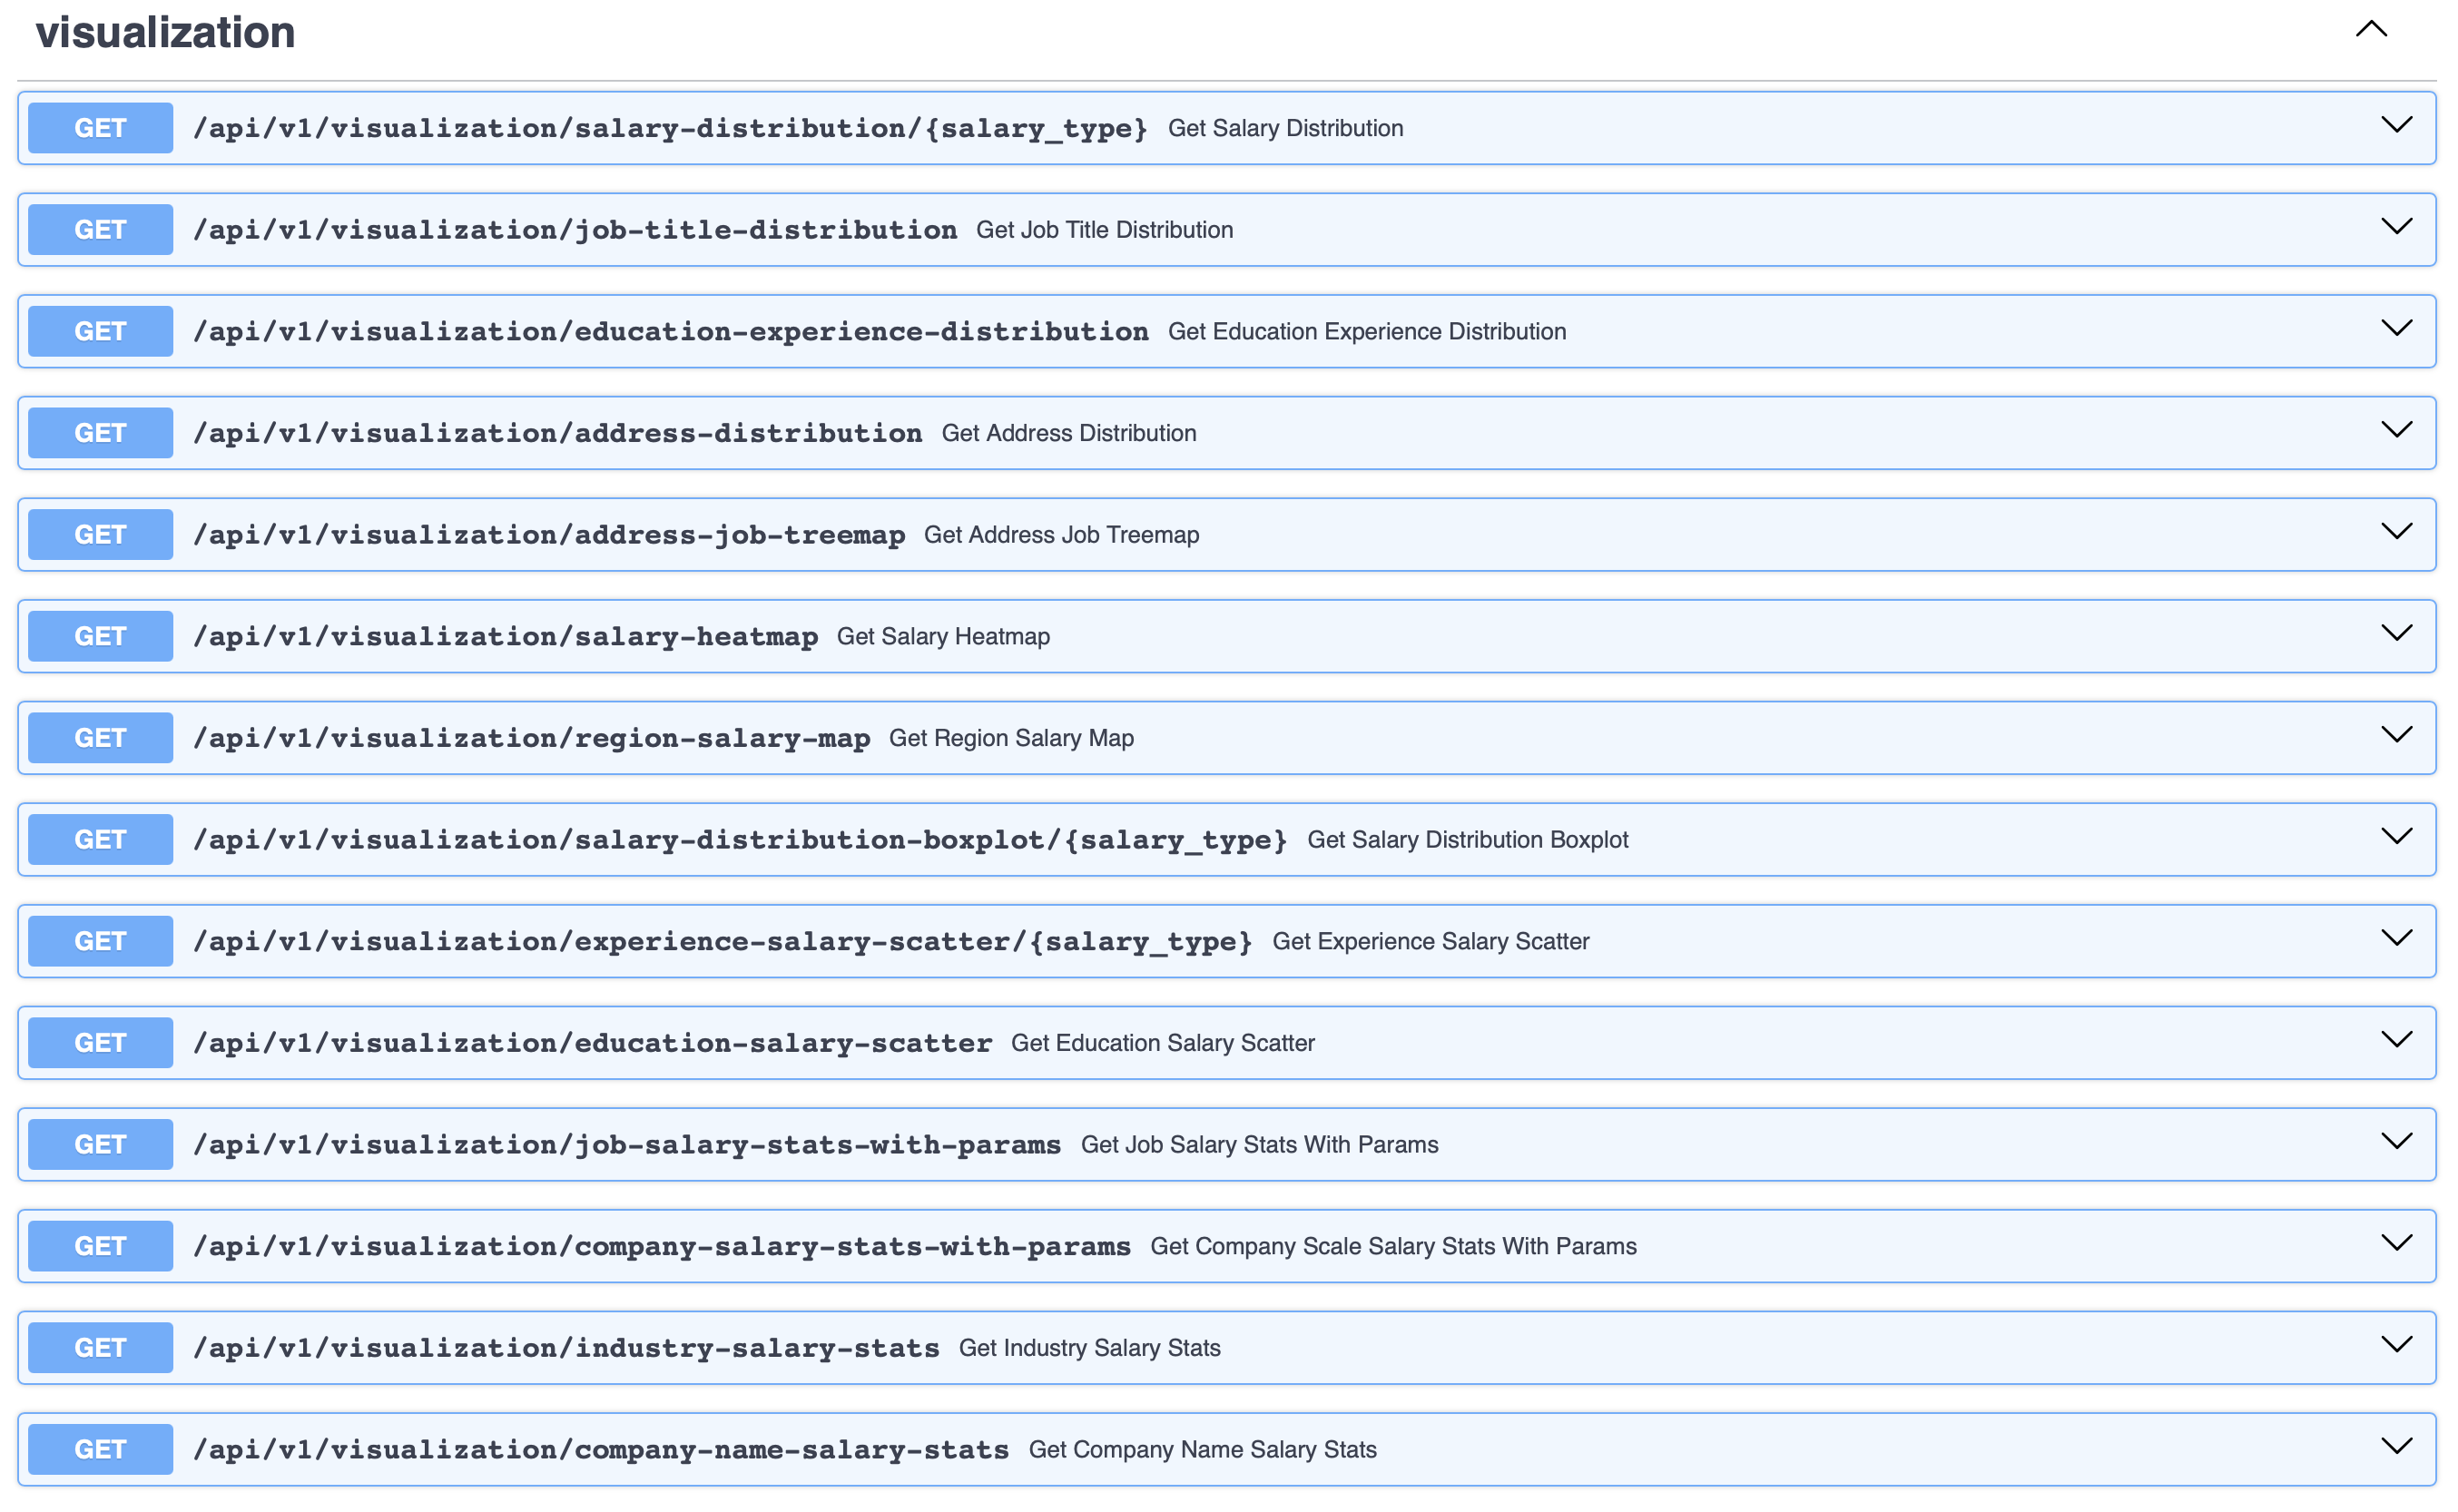
\includegraphics[width=0.9\textwidth]{figures/visualization_api.png}
    \caption{可视化模块API接口文档}
    \label{fig:visualization_api}
\end{figure}

\subsubsection{监控模块(/monitor)}
监控模块提供系统运行状态和数据质量的监控接口:

\begin{itemize}
    \item \textbf{数据质量监控}:
    \begin{itemize}
        \item 路径:\texttt{/monitor/data-quality}
        \item 方法:GET
        \item 功能:监控数据的完整性和质量
    \end{itemize}
    
    \item \textbf{数据一致性监控}:
    \begin{itemize}
        \item 路径:\texttt{/monitor/data-consistency}
        \item 方法:GET
        \item 功能:检查数据的一致性和完整性
    \end{itemize}
    
    \item \textbf{ETL进度监控}:
    \begin{itemize}
        \item 路径:\texttt{/monitor/etl-progress}
        \item 方法:GET
        \item 功能:监控ETL处理的进度
    \end{itemize}
    
    \item \textbf{系统性能监控}:
    \begin{itemize}
        \item 路径:\texttt{/monitor/system-performance}
        \item 方法:GET
        \item 功能:监控系统的性能指标
    \end{itemize}
\end{itemize}